%% ==============================
\chapter{Introduction}
\label{sec:introduction}
%% ==============================
Questions to ask:
\begin{enumerate}
    \item What is your research topic? (From wide to narrow scope)
    \item What is the research problem or gap in the field that this work aims to address?
    \item Why is this problem or gap important?
    \item What are the research questions or hypotheses? 
    \item What is the scope of your work? (What are the limitations?)
    \item How is the following work structured?
\end{enumerate}

\begin{enumerate}
    \item General field of path planning for mobile robots
    \item Problem of path planning in multi-story environments
    \item Shared human-robot spaces
    \item Research question: How to plan in a multi-story environment? And how to drive in public spaces with service robots?
    \item Significance: Many use cases in public spaces in large hierarchical environments like hospitals.
    \item Development of a global planner plugin for straight and predictable paths in multi-story environments.
    \item Structure of the thesis
\end{enumerate}

%% ==============================
\section{Motivation}
\label{sec:motivation}
%% ==============================
The research area of autonomous mobile robotics deals with all sub-areas that are necessary to ensure the required degree of autonomy and mobility for specific tasks. In addition to navigation and manipulation, this also includes the perception of the environment as well as the internal state. Autonomous mobile robots form a combination of the disciplines of electrical engineering, mechanical engineering and computer science. Computer science in particular is rapidly driving current developments. Complex algorithms for localisation and navigation enable the necessary mobility. Artificial intelligence offers robust methods for image processing, object recognition and voice control through neural networks and machine learning. \todo{Quelle überpüfen und aktualisieren} According to the market research company Gartner, autonomous robotics is the most important strategic technological trend of 2019 \cite{Cearley.2018} and number eight in 2020 \todo{Quelle} In recent years it has only been superseded by new developments in the field of AI. The market for service robots is also growing rapidly. \todo{Quelle aktualisieren} According to the International Federation of Robotics, the market volume for service robots in 2018 was 9.2 billion US dollars \cite{InternationalFederationofRobotics.2019}. The market volume is expected to grow to 46.2 billion US dollars by 2025 \cite{InternationalFederationofRobotics.2019}.

Especially in the application area of service robotics, tasks are becoming increasingly complex. The best-known are household robots that, for example, take care of vacuuming or mow the lawn. However, more extensive tasks such as support in everyday life by folding the laundry \todo{Quelle}, can now also be taken over by assistance robots. The commercial application of service robots is mostly limited to isolated tasks without the need to interact with humans. Another application area are robots that operate in strictly defined spaces separted from humans, for example robots for material logistics in warehouses or production facilities. There are af few start-ups which are trying to establish service robots in public spaces as well \todo{Quelle hinzufügen CareoBot}. However, the development of service robots for public spaces is still in its infancy. The main reason for this is the complexity of the tasks and the environment. In addition to the technical challenges, there are also legal and ethical issues that need to be addressed.

%% ==============================
\section{Problem Statement}
\label{sec:problem_statement}
%% ==============================
Mobile robots are increasingly being used in large environments, such as hospitals, to improve efficiency and reduce human workload. However, navigating over multiple stories poses a significant challenge for mobile robots, as it requires a planner that can account for complex spatial configurations and still find the shortest path. Moreover, the planned path must be straight, deterministic and predictable for humans who could be walking in the same space as the robot. Therefore, the specific research problem addressed in this thesis is the development of a planner that can enable a mobile robot to navigate over multiple stories in large environments, while ensuring a straight, deterministic and human-predictable path. 

The ability to navigate over multiple stories is important for mobile robots in large environments, as it can significantly increase their utility and effectiveness. For instance, in hospitals, mobile robots could be used for tasks such as delivering medicines, transporting equipment, or guiding patients and visitors. Although for specific use-cases proprietary solutions exist, the lack of an open-source planner for multi-story navigation is a major bottleneck in the development of mobile robots for service applications. Moreover, the need for a straight, deterministic and human-predictable path is essential for ensuring safety and reducing the risk of collisions or accidents in shared human-robot spaces.

The two main research questions addressed in this thesis are:
\begin{enumerate}
    \item How to navigate in large multi-story environments?
    \item How to plan paths that are straight, deterministic and human-predictable?
\end{enumerate}

The scope of this work is limited to developing a planner which plans a priori with previously gathered information, in contrast to a controller which follows the planned path and adapts to dynamic obstacles. The main assumption is that the a map of the whole environment is previously recorded and provides a complete representation of the plannable space.

%% ==============================
\section{Use case PeTRA}
\label{sec:use_case}
%% ==============================
The use case of this work is a mobile robot that is used to support patient logistics in care facilities. This includes tasks such as delivering medicines and transporting a patient to their examiniations. This work is part of the \gls{petra} research project, which aims to develop a mobile robot for autonomously transporting patients in a hospital and completing other service tasks. \gls{petra} is funded by the \gls{bmbf} and developed at the \gls{iras} of the \gls{hka}.

\todo{This is a copy from IAS-18 rephrase!}Transporting patients from ward to examination is part of the daily routine in a hospital. This manual transport is currently also performed by trained nurses, who are absent from the ward during this time and cannot perform nursing activities. To save time, patients are moved through the hospital mainly in beds, even though some of them are able to walk by themselves. The currently used transfer method neither promotes the patients' mobility nor allows them to decide for themselves whether and how they want to walk. The BMBF-funded research project of which this work is a part, is developing a Person Transfer Robot Assistant (PeTRA) to solve these problems. The goal is to relieve caregivers from time-consuming and labor-intensive person transfers in order to have more time for qualitative care \cite{petra-konsortium_personen-transfer_2022}. For this task, an autonomous mobile robot was developed in close collaboration with three hospitals. PeTRA offers different transfer modes, which each patient can use individually as needed, see figure  \ref{fig:multi_mobility_methods}. Autonomous patient transport is realized with sensory coupling for free walking or with the support of a rollator (center) and a modular platform for wheelchairs (left). This platform is used for safe wheelchair transport and can be coupled. In addition, an integrated robotic arm performs service tasks (right). These include, for example, the transport of drugs or blood samples between the storage area and the wards..

\begin{figure}[h]
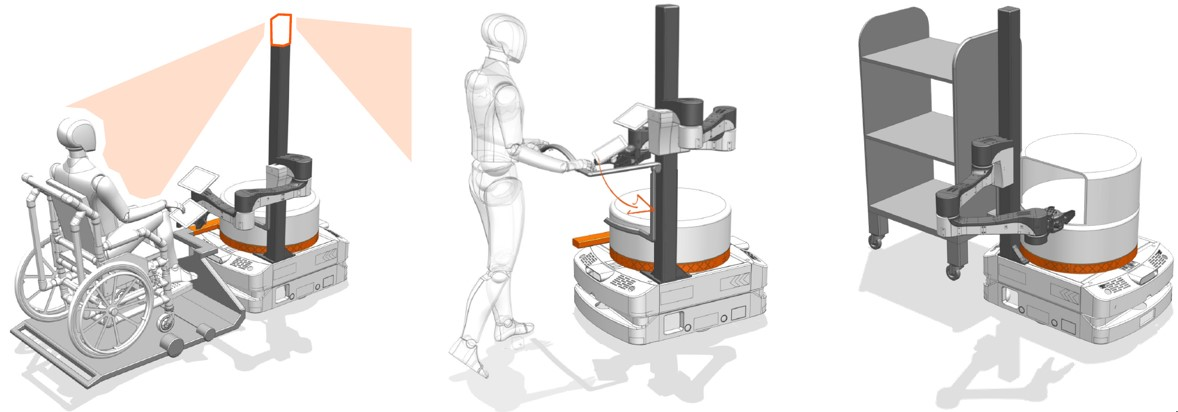
\includegraphics[width=\textwidth]{figures/02_state_of_the_art/PeTRA_transport_modes.jpg}
\caption[]{Multi-mobility methods of PeTRA: Wheelchair transport (left), sensory coupling (center) and material transport (right).}
\centering
\label{fig:multi_mobility_methods}
\end{figure}


%% ==============================
\section{Structure of this Thesis}
\label{sec:structure}
%% ==============================
The following work is structured as follows: Chapter \ref{sec:state_of_the_art} provides an overview of the state of the art in the field of multi-story path planning for mobile robots. It also discusses the limitations of existing approaches. Chapter \ref{sec:methods} describes the methodology used to address the research questions. The concept of the graph-based planner is presented in Chapter \ref{sec:concept} followed by the implementation in Chapter \ref{sec:implementation}. This shows the approaches of creating a graph from a previously recorded map. Chapter \ref{sec:results} presents the results of the work. Chapter \ref{sec:discussion} discusses the results and provides recommendations for future work. Chapter \ref{sec:conclusion} concludes the thesis.